\documentclass[10pt]{article}

\usepackage{amsmath}
\usepackage{amssymb}
\usepackage{graphicx}
\usepackage[margin=0.75in]{geometry}

\setlength{\parindent}{0pt}
\setlength{\parskip}{4pt}

\begin{document}

\begin{center}
{\Large\textbf{ZMP-Based Stability Cost Formulation}}
\end{center}

\section*{1. Ground Contact Force and Moment}

The total mass and centre of mass are

\begin{equation}
m=\sum_i m_i,
\qquad
p_C=\frac{1}{m}\sum_i m_i p_{C,i}.
\end{equation}

The angular momentum about the centre of mass is

\begin{equation}
H_C=
\sum_i
\left[
R_iI_i\omega_i^B+
(p_{C,i}-p_C)\times m_i(\dot p_{C,i}-\dot p_C)
\right].
\end{equation}
where $\omega$ is angular velocity and $I$ is inertia of each components.

The total ground force and moment are

\begin{equation}
F=m(\ddot p_C+ge_3),
\qquad
M_O=\dot H_C+p_C\times F.
\end{equation}

where $e_3=[0,0,1]^T$ is an upward unit vector

\section*{2. Zero-Moment Point}

For a horizontal ground surface,

\begin{equation}
x_Z=-\frac{M_{O,y}}{F_z},
\qquad
y_Z=\frac{M_{O,x}}{F_z},
\qquad F_z>0.
\end{equation}

With $p_C=[x_C,y_C,z_C]^T$,

\begin{equation}
\boxed{
x_Z=
x_C-
\frac{z_Cm\ddot x_C+\dot H_{C,y}}
{m(g+\ddot z_C)}
}
\end{equation}

\begin{equation}
\boxed{
y_Z=
y_C-
\frac{z_Cm\ddot y_C-\dot H_{C,x}}
{m(g+\ddot z_C)}
}.
\end{equation}

\section*{3. Stability Cost}

Let $a$ and $b$ be the half-length and half-width of the support
region. The ZMP constraint with safety margin $\delta$ is

\begin{equation}
|x_Z|\leq a-\delta,
\qquad
|y_Z|\leq b-\delta.
\end{equation}

Define the instantaneous stability cost as

\begin{equation}
\boxed{
L=
\left(\frac{x_Z}{a}\right)^2+
\left(\frac{y_Z}{b}\right)^2
}.
\end{equation}

Thus, $L=0$ at the support centre and increases as the ZMP moves
toward the support boundary.

For $N$ samples, the total stability cost is

\begin{equation}
\boxed{
J=\frac{1}{N}\sum_{k=1}^{N}L_k
}.
\end{equation}

The control input is defined as:
\begin{equation}
\boxed{
u=
\begin{bmatrix}
a_{\mathrm{ref}}\\
\tau_A\\
\omega_{W,\mathrm{ref}}
\end{bmatrix}
.
}
\end{equation}
Here, $a_{\mathrm{ref}}$ is linear actuator position,
$\tau_A$ contains the arm joint torque commands, and
$\omega_{W,\mathrm{ref}}$ contains the four wheel-speed references
for the AK80-9 motors in MIT velocity-tracking mode.

The control objective is therefore

\begin{equation}
\boxed{
\min_u J
}
\end{equation}

subject to the ZMP, task, and actuator constraints.

\section*{4. Block Diagram}
\begin{figure}[h]
\centering
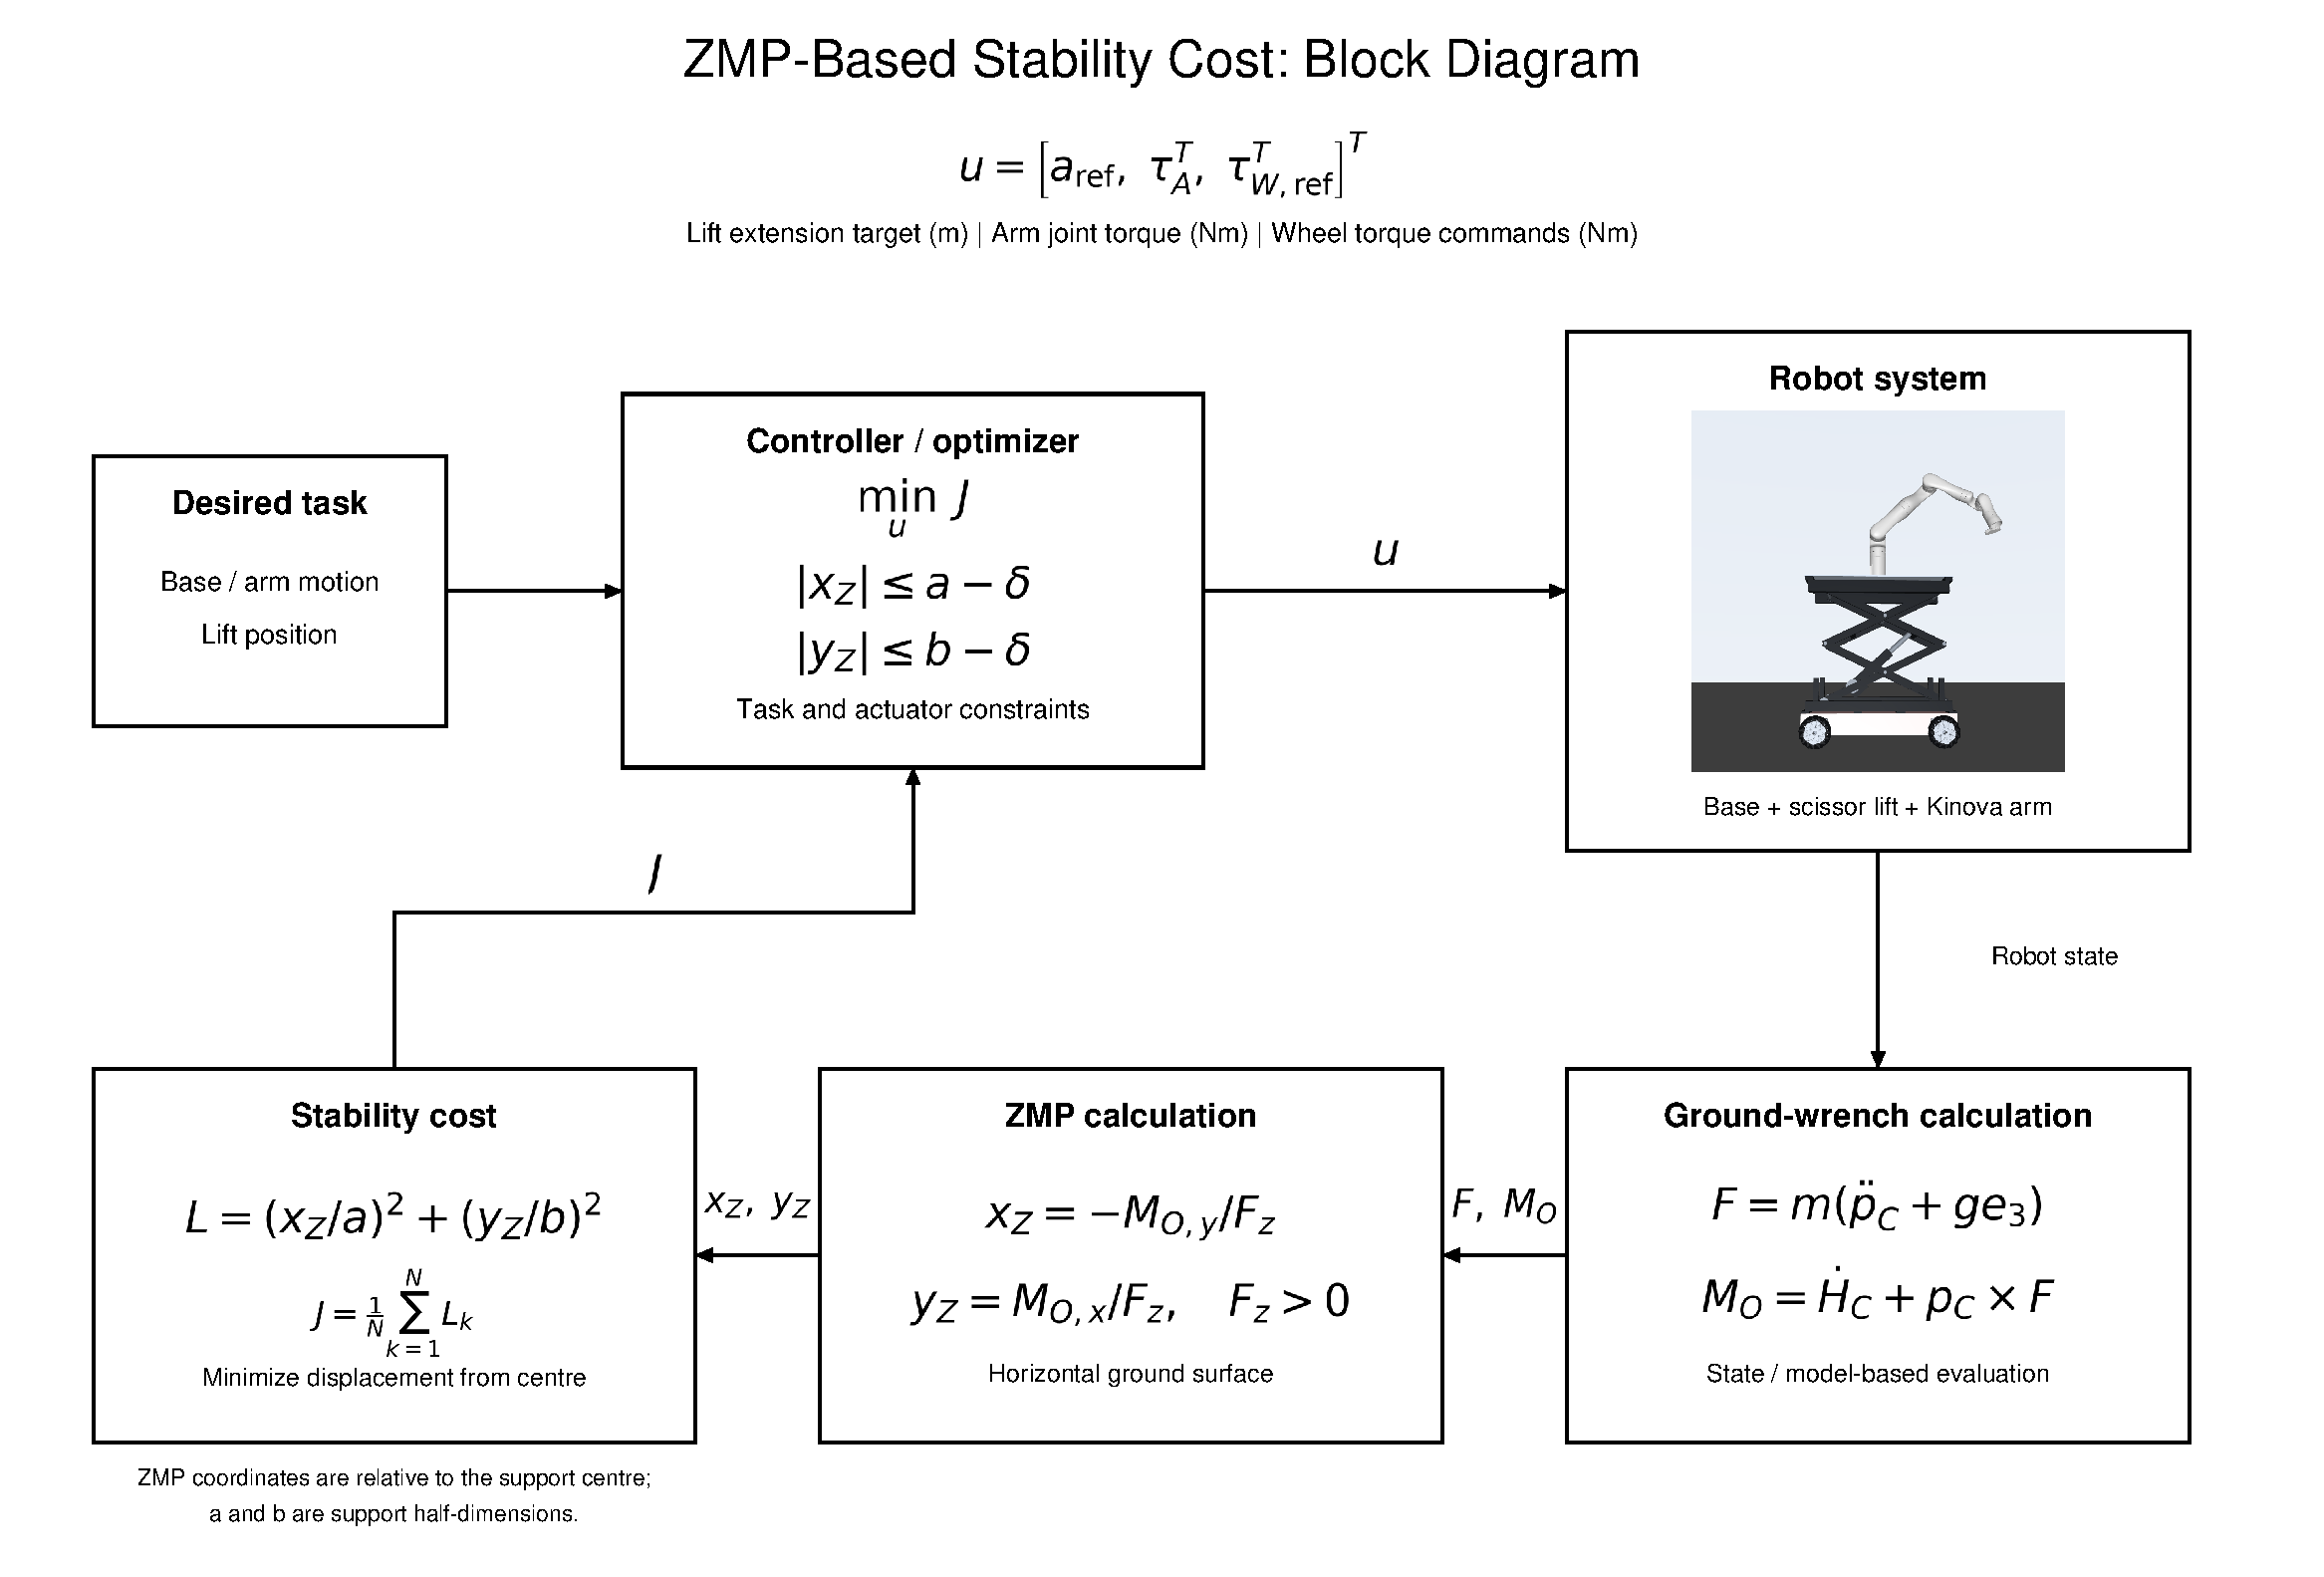
\includegraphics[width=\linewidth]{zmp_final_block_diagram.pdf}
\caption{Block diagram corresponding to the cost function.}
\end{figure}

\end{document}
